% sizes tiny scriptsize footnotesize small normalsize large Large LARGE huge Huge

\documentclass[presentation]{beamer}

\usetheme{JuanLesPins}
\usecolortheme{orchid}
\setbeamertemplate{headline}{}
\setbeamertemplate{navigation symbols}{}

\usepackage{subfig}
\usepackage{graphicx}
\usepackage[english]{babel}
\usepackage[latin1]{inputenc}
\usepackage{color}
\usepackage{listings}
\usepackage{textcomp}
\usepackage{csquotes}
\usepackage{ragged2e}
\definecolor{mygreen}{rgb}{0,0.6,0}
\definecolor{mygray}{rgb}{0.5,0.5,0.5}
\definecolor{mymauve}{rgb}{0.58,0,0.82}

\lstset{
  backgroundcolor=\color{white},   % choose the background color; you must add \usepackage{color} or \usepackage{xcolor}; should come as last argument
  basicstyle=\footnotesize\ttfamily, % the size of the fonts that are used for the code
  breakatwhitespace=false,         % sets if automatic breaks should only happen at whitespace
  breaklines=true,                 % sets automatic line breaking
  captionpos=b,                    % sets the caption-position to bottom
  commentstyle=\color{mygreen},    % comment style
  deletekeywords={...},            % if you want to delete keywords from the given language
  escapeinside={\%*}{*)},          % if you want to add LaTeX within your code
  extendedchars=true,              % lets you use non-ASCII characters; for 8-bits encodings only, does not work with UTF-8
  frame=single,	                   % adds a frame around the code
  keepspaces=true,                 % keeps spaces in text, useful for keeping indentation of code (possibly needs columns=flexible)
  keywordstyle=\color{blue},       % keyword style
  morekeywords={*,...},            % if you want to add more keywords to the set
  numbers=none,                    % where to put the line-numbers; possible values are (none, left, right)
  numbersep=5pt,                   % how far the line-numbers are from the code
  numberstyle=\tiny\color{mygray}, % the style that is used for the line-numbers
  rulecolor=\color{black},         % if not set, the frame-color may be changed on line-breaks within not-black text (e.g. comments (green here))
  showspaces=false,                % show spaces everywhere adding particular underscores; it overrides 'showstringspaces'
  showstringspaces=false,          % underline spaces within strings only
  showtabs=false,                  % show tabs within strings adding particular underscores
  stepnumber=2,                    % the step between two line-numbers. If it's 1, each line will be numbered
  stringstyle=\color{mymauve},     % string literal style
  tabsize=2,	                   % sets default tabsize to 2 spaces
  title=\lstname,                  % show the filename of files included with \lstinputlisting; also try caption instead of title
  linewidth=10.7cm,
}

\usepackage{tikz}
\usetikzlibrary{positioning}


% Add any additional packages you use in your presentation
% -----pack
% \usepackage{xxx}
% -----

% Add your custom definitions etc., if required
% -----misc
% \newcommand{\xxx}[1]{[#1]}
% -----




\title{Data-flow analysis}
\subtitle{Symbolic interpretation, Data-flow equations}
\author[]{Michal Barczyk, Michal Cyrkowski}
\institute[]{}
\date{}


\begin{document}

\begin{frame}
  \titlepage
\end{frame}

\begin{frame}
  \frametitle{Methods of collecting context information from AST}
  
%   \begin{definition}
% A prime number is a number that...
% \end{definition}

\begin{block}{Control-flow graph}
\justify{For each AST node we need to know its flow-of-control successor(s). We can represent it as an additional data structure where every node has pointer or pointers to its flow-of-control successor. Pointers can be visualised on orginal AST.}
\end{block}

\begin{block}{Threading the tree}
\justify{Threading is a method of constructing control-flow graph. For each node threading routine detects production describing node and calls threading routine on its children recoursively. Each instance of threading routine is aware of global variable \emph{last\_node\_pointer} pointing to the last node processed on the controlflow
path.}
\end{block}
   
\end{frame}

\begin{frame}
  \frametitle{Threading the AST}
  \begin{block}{}
    \justify{Using this technique, the threading routine for a binary expression could, for example, have the following form:} 
    
    \lstinputlisting[language=Python]{procedure1.py}
    
    \justify{This makes the present node the successor of the last node of the right operand and then registers it as the next dynamically last node.}
  \end{block}
  


  
\end{frame}

\begin{frame}
  \frametitle{Threading the AST}
  
   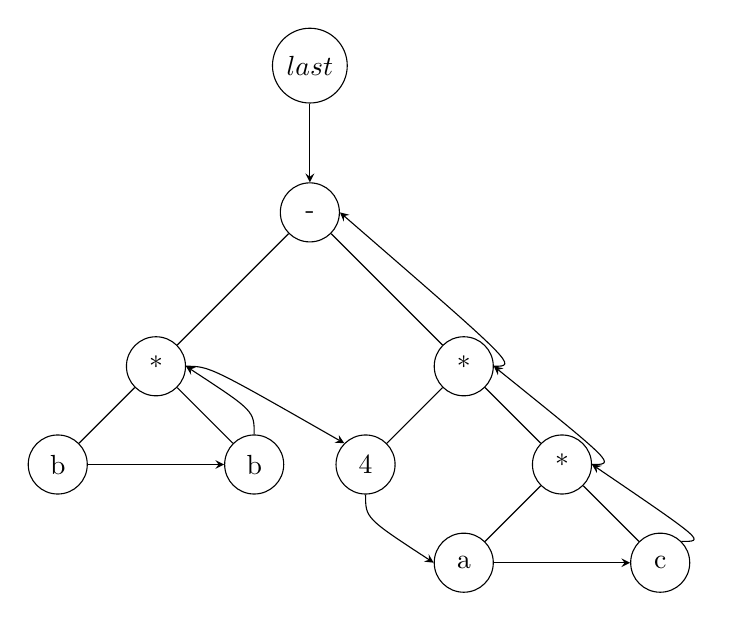
\begin{tikzpicture}[>=stealth, every node/.style={circle, draw, minimum size=0.75cm}]
   
        %Nodes
        \node   (last) {$last$};
        \node   (minus) [below=1 of last] {-};
        \node   (star1) [below left=2 of minus] {*};
        \node   (b1) [below left=1 of star1] {b};
        \node   (b2) [below right=1 of star1] {b};
        \node   (star2) [below right=2 of minus] {*};
        \node   (four) [below left=1 of star2] {4};
        \node   (star3) [below right=1 of star2] {*};
        \node   (a) [below left=1 of star3] {a};
        \node   (c) [below right=1 of star3] {c};
        
        
        %Lines
        \draw[-] (minus.south west) -- (star1.north east);
        \draw[-] (minus.south east) -- (star2.north west);
        \draw[-] (star1.south west) -- (b1.north east);
        \draw[-] (star1.south east) -- (b2.north west);
        \draw[-] (star2.south west) -- (four.north east);
        \draw[-] (star2.south east) -- (star3.north west);
        \draw[-] (star3.south west) -- (a.north east);
        \draw[-] (star3.south east) -- (c.north west);
        
        \draw[->] (b1.east) .. controls +(right:3mm)  .. (b2.west);
        \draw[->] (b2.north) .. controls +(up:3mm)  .. (star1.east);
        \draw[->] (star1.east) .. controls +(right:3mm)  .. (four.north west);
        \draw[->] (four.south) .. controls +(down:3mm)  .. (a.west);
        \draw[->] (a.east) .. controls +(right:3mm)  .. (c.west);
        \draw[->] (c.north east) .. controls +(right:3mm)  .. (star3.east);
        \draw[->] (star3.east) .. controls +(right:3mm)  .. (star2.east);
        \draw[->] (star2.east) .. controls +(right:3mm)  .. (minus.east);
        
        \draw[->] (last.south) .. controls +(down:3mm)  .. (minus.north);
    
    \end{tikzpicture}
  
  Control flow graph for $b*b-4*a*c$ \\(flow order marked with arrows after threading)


\end{frame}

\begin{frame}
  \frametitle{Threading the AST}
  \begin{block}{Problems}
  \justify{The problem occurs if the flow of control exists in more than one place. The perfect example is if/else statment that causes two problems. The first is that node that corresponds to the run-time then/else decision has two successors rather than one. The second is that when we reach the node dynamically following the entire if-statement, its address must be recorded in the dynamically last nodes of both the then-part and the else-part. As a result single variable \emph{last\_node\_pointer} is no longer sufficient.}
  \end{block}
  
\end{frame}

\begin{frame}
  \frametitle{Threading the AST}
  \begin{block}{First problem solution}
  \justify{This issue can be simply solved  by storing pointers to two successors in the if-node.}
  \end{block}
  
  \begin{block}{Second problem solution}
  \justify{One way to solve the second problem is to replace \emph{last\_node\_pointer} by a set of last nodes that will be filled in when next node in the control-flow path is dynamically found.\\
  Another method is to construct a special join node to merge the diverging flow of control. Such node is part of control-flow graph without being part of AST.}
  \end{block}
  
\end{frame}

\begin{frame}
  \frametitle{Methods of collecting context information from AST}
  
  \lstinputlisting[language=Python]{procedureIf.py}
  
\end{frame}

\begin{frame}
  \frametitle{Methods of collecting context information from AST}
  
  \begin{tikzpicture}[>=stealth, every node/.style={circle, draw, minimum size=0.75cm}]
  
    
    \node   (if) {$if$};
    \node (x) [left=2 of if] {$X$}
    \node   (cond) [below left=1.5 of if] {$condition$};
    \node   (then) [below =1.5 of if] {$then$};
    \node   (else) [below right=1.5 of if] {$else$};
    \node   (endif) [below right=1.5 of then] {$end\;if$};
    \node   (last) [above right=4 of endif] {$last$};
    
    \draw[<-] (if.south west) .. controls +(left:3mm)  .. (cond.north);
    \draw[->] (if.south) .. controls +(down:3mm)  .. (then.north);
    \draw[->] (if.south east) .. controls +(right:3mm)  .. (else.north);
    \draw[->] (then.south) .. controls +(down:3mm)  .. (endif.west);
    \draw[->] (else.south) .. controls +(down:3mm)  .. (endif.north);
    \draw[->] (last.south) .. controls +(down:3mm)  .. (endif.east);
    
    \end{tikzpicture}
    \newline
    \newline
    AST and control-flow graph of an if-statement after threading
  
\end{frame}

\begin{frame}
  \frametitle{Symbolic interpretation}
  
  \begin{block}{Symbolic interpretation}
  \justify{During program execution, the control follow one possible path through the control-flow graph. The behaviour of a code block is determined by the values of the variables created/assigned before execution of this block and this block can change values of variables determining a following execution (path in control-flow graph). Much contextual information about variables can be deduced statically by
  simulating process of execution at compile
  time.This technique is called \textbf{symbolic interpretation} or simulation on the stack.}
  \end{block}
  
\end{frame}

\begin{frame}
  \frametitle{Symbolic interpretation}
  \begin{block}{Stack representation in control-flow graph of if-statement}
  \justify{In this example we assume that we arrive with a stack containing two variables x and y.\\
  x is initialized and y is valued 5. The condition is y $>$ 0.}
  \end{block}
  \begin{center}
      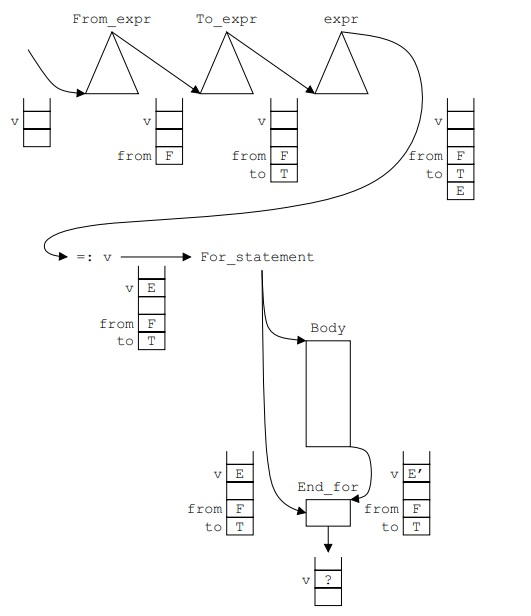
\includegraphics[scale=0.45]{510.jpg}
  \end{center}
\end{frame}

\begin{frame}
  \frametitle{Simple symbolic interpretation}
  
  \begin{block}{Simple symbolic interpretation}
  \justify{\textbf{Simple symbolic interpretation} allows us to check for the use of uninitialized variables. In order to do it, we create compile-time representation of the local stack as list of pairs \emph{(name, property)}}. 
  \begin{itemize}
    \item At the beginning property list is empty or contains parameters with properties since parameters are obviously initialized.
    \item Then we follow the path on control-flow graph processing encountered varibles.
    \item When a declaration is met, the declared name is added to the property list with status: initialized or uninitialized.
    
    \end{itemize}
 
  \end{block}
  
\end{frame}

\begin{frame}
  \frametitle{Simple symbolic interpretation}
  
  \begin{block}{Simple symbolic interpretation}
  \begin{itemize}
    \item When the control-flow splits (eg. if-node) there is made a copy of property list and simulated execution is done for then-part and for else-part.
    \item When an assignment is met, the status of the destination variable is set to
    initialized, after processing the source expression first, since it may contain the same
    variable.
    \item When the variable is used (eg. in expression), its status is checked in property list. If its status is uninitialized/possibly uninitialized we are given error/warning.
    \end{itemize}
 
  \end{block}
  
\end{frame}

\begin{frame}
  \frametitle{Simple symbolic interpretation}
  
  \begin{block}{Stack representations in the control-flow graph of a for loop}
  \justify{When the interpreter meets a for statement it passes through the bands and the inintalization of the controlled variable. It then makes a copy of the list which is called the \textbf{loop-exit list}. This list collects the information at the exit of the loop.\\}
  \begin{itemize}
      \item If loop-exit statement is found inside the loop the callected list is merged into loop-exit list and interpretation continues with empty list.\\
      \item If return statement is found inside loop or we reach the end of the routine present list is merged into loop-exit list and interpretation sontinues with empty list.
  \end{itemize}
  \end{block}
  
\end{frame}

\begin{frame}
  \frametitle{Simple symbolic interpretation}
  \begin{block}{Stack representations in the control-flow graph of a for loop}
  \begin{itemize}
      \item If return statement is found outside loop interpreter can raise an error.
      \item If the end of the routine node is reached interpreter checks all variable identifiers in the list. If on has status \emph{Uninitialized} it never was initialized and a warning can be given.
  \end{itemize}
  \justify{
  \textbf{Note that the interpreter ignores the back jump of the for-statement}.}
  \end{block}
  
\end{frame}

\begin{frame}
  \frametitle{Simple symbolic interpretation}
  \begin{block}{Simple symbolic interpretation requirements}
  \begin{itemize}
      \item The program must consist of flow-of-control structures with one entry point and one exit point only.
      \item The values of the property must form a lattice, which means that the values can be ordered in a sequence $v_1...v_n$ such that there is no operation that will transform $v_j$ into $v_i$; we will write $v_i < v_j$ for all $i<j$.
      \item The result of merging two values must be at least as large as the smaller of the two.
      \item An action taken on $v_i$ in a given situation must make any action taken on $v_j$ in the same situation superfluous, for $v_i \leq v_j$.
  \end{itemize}
  \end{block}
  \begin{block}{}
  \justify{If this four requirements are not fulfilled it is necessary to preform \textbf{full symbolic interpretation} that avoids above shortcuts.}
  \end{block}
\end{frame}

\begin{frame}
  \frametitle{Full symbolic interpretation}
  \begin{block}{Full symbolic interpretation}
  \justify{Goto statements cannot be handled by simple symbolic interpretation, since they
violate requirement 1 from the previous slide. In order to handle them, we use \textbf{full symbolic interpretation}}. 
  
  \end{block}
  
  \begin{block}{Algorithm}
  \justify{
  \textbf{Full symbolic interpretation} consists of performing the simple symbolic interpretation algorithm repeatedly until properties stop changing. Instead of one property list, we need separate list for each label (a place algorithm can go to) in the routine. We perform the simple symbolic interpretation algorithm as before, adding \textbf{special actions} at goto-jumps and labels.}
  \end{block}
  
\end{frame}

\begin{frame}
  \frametitle{Full symbolic interpretation}
  
  \begin{block}{Algorithm}
  Special actions mean:
  \begin{itemize}
      \item Each time we meet a
jump to a label $L$, we merge our present list into L\textquotesingle s list and continue with the empty
    \item When we meet the label $L$ itself, we merge in our present list, and continue with
the merged list.
  \end{itemize}
  \justify{It looks like we have a list of situations at all positions label $L$ can be reached from (for each label $L$). Actually, it is not so easy, because we have to consider a following situation: 

If we first meet the label $L$ and then a jump to it, the list at $L$ was not complete,
since it may be going to be modified by that jump. To solve it, when we are at the end of the
routine, we have to run the simple symbolic interpretation algorithm again, using the
lists we have already created for the labels. We have to repeat this, until none of properties
changes any more.}
 
  \end{block}
  
\end{frame}

\begin{frame}
  \frametitle{Data-flow equations}
  \begin{block}{Data-flow equations}
  \justify{Data-flow equations are a half-way automation of full symbolic interpretation, in
which the stack representation is replaced by a collection of sets, the semantics of a
node is described more formally, and the interpretation is replaced by a built-in and
fixed propagation mechanism.}
  \end{block}
  \begin{block}{Stacks replacement}
  Stack is replaced by two variable sets:\\
  \begin{itemize}
      \item $IN(N)$, representation of node N input
      \item $OUT(N)$, represtentation of node N output
  \end{itemize}
  Both $IN(N)$ and $OUT(N)$ start of empty and are computed by propagation mechanisem.
  \end{block}
\end{frame}

\begin{frame}{Data-flow equations}
    \begin{block}{Semantics description}
     In order to describe semantics for each node N two constatn sets are defined:
     \begin{itemize}
         \item $GEN(N)$
         \item $KILL(N)$
     \end{itemize}
     Their contents are derived from the information in the node.
    \end{block}
\end{frame}

\begin{frame}
  \frametitle{Data-flow equations}
  \begin{block}{Setting up the data-flow equations}
  \justify{When control passes through node $N$ at run time, the state of the program is probably changed. This change causes the removal of some items from the set at $N$ and the addition of some other items during compilation. We keep removed and added items in separated sets: the set $KILL(N)$ contains the items removed by the
node $N$ and the set $GEN(N)$ contains the items added by the node. For instance,
item in a GEN set could be \enquote{Variable $x$ is equal to variable $y$ here}
for the assignment node $x:=y$. The same node has the item \enquote{Variable $x$ is equal to
any value here} in its KILL set, which is actually a finite representation of an infinite set of items.}
  \end{block}
  
\end{frame}

\begin{frame}
  \frametitle{Data-flow equations}
  \begin{block}{Data-flow equations for node $N$}
 
  $IN(N) = \bigcup\limits_{M \;= \; dynamic \;predecessor\;of\;N} OUT(M)$
    \newline
    \newline
    \newline
  $OUT(N) = (IN(N) \setminus KILL(N)) \cup GEN(N)$
  
  \end{block}
  
  \begin{block}{Data-flow equations interpretation}
  \justify{The first data-flow equation tells us how to obtain the IN set of all nodes when we
know the OUT sets of all nodes, and the second data-flow equation tells us how
to obtain the OUT set of a node if we know its IN set (and its GEN and KILL
sets, but they are constants). This suggests \textbf{closure algoritm} for establising the values of $IN(N)$ and $OUT(N)$ sets.}
  \end{block}
  
\end{frame}

\begin{frame}
  \frametitle{Solving data-flow equations}
  \begin{block}{Closure algorithm}
  Data definitions:
  \begin{itemize}
      \item Constant $KILL(N)$ and $GEN(N)$ sets
      \item Variable $IN(N)$ and $OUT(N)$ sets
  \end{itemize}
  Initializations:
  \begin{itemize}
      \item The IN set of the top node is initialized with information established externally
      \item For all other nodes N, IN(N) and OUT(N) are set to empty
  \end{itemize}
  Inference rules:
  \begin{itemize}
      \item  For any node N, $IN(N)$ must contain
      \item For any node N, $OUT(N)$ must contain
  \end{itemize}
  
  \end{block}
\end{frame}

\begin{frame}
  \frametitle{Solving data-flow equations}
  \begin{block}{Closure algorithm implementation}
  \justify{The closure algorithm can be implemented by traversing the control graph repeatedly and computing the $IN(N)$ and $OUT(N)$ sets of the nodes visited. Once we have performed a complete traversal of the control-flow graph in which no $IN(N)$ or $OUT(N)$
set changed, we have found the solution to the set of equations. We then know the
values of the $IN$ sets of all nodes and can use this information for context checking
and code generation.}
  \end{block}
\end{frame}

\begin{frame}
  \frametitle{Interprocedural data-flow analysis}
  \begin{block}{Interprocedural data-flow analysis}
  \justify{Interprocedural data flow is the data flow between routines, as opposed to that
inside routines. Such data flows in two directions, from the caller to the callee in a
routine call, and from callee to caller in a return statement. The resulting information
seldom serves context checking and is mostly useful for optimization purposes.}
  \end{block}
\end{frame}

\begin{frame}
  \frametitle{Carrying the information upstream}
  \begin{block}{Live analysis}
  \justify{Both symbolic interpretation and data-flow equations collect information from the preceding
nodes and can deposit it at the present node. Nonetheless,
there are some items of interest that can be determined best (or only) by following
the control-flow \textbf{backwards}. One example of such information is the
liveness of variables. A variable is live at a given node $N$ in the control-flow graph if
the value it holds is used on at least one path further through the control-flow graph
from node $N$ - otherwise it is dead.
During code generation it is important to know if a variable is live or dead at a
given node in the code, since if it is dead, the memory allocated to it can be reused.}
\end{block}
  
\end{frame}

\begin{frame}
  \frametitle{Carrying the information upstream}
  \begin{block}{Live analysis}
\justify{The start of the live range of a variable $V$ is marked by a node that contains value of $V$ definition. The end of the live range is marked by a node that contains the last
use of the value of V. The problem is that it is hard to recognize this node.
Information about the future use of variable values cannot be obtained in a
straightforward strategy using symbolic interpretation or dataflow
equations. Fortunately, this methods can be modified so they can solve this and
other \enquote{backward flow} problems. }
 \end{block}
  
\end{frame}



\begin{frame}
  \frametitle{Live analysis by symbolic interpretation}
  \begin{block}{}
  \justify{Since symbolic interpretation follows the control-flow graph, it has no way of looking ahead and finding out if there is another use of the value of a given variable V,
and so it has no way to set some isLastUseOfV attribute of the node it is visiting.
The general solution to this kind of problem is to collect the addresses of the values
we cannot compute and to fill them in when we can. Such lists of addresses are
called \textbf{backpatch lists} and the activity of filling in values when the time is ripe is
called \textbf{backpatching}.}
  \end{block}
\end{frame}

\begin{frame}
  \frametitle{Live analysis by symbolic interpretation}
  \begin{block}{Backpatching}
  \justify{Backpatching means that for each variable V we keep in our stack
representation a set of pointers to nodes that contain the latest, most recent uses of
the value of V; note that when looking backwards from a node we can have more
than one most recent use, provided they are along different paths. Now, when we
arrive at a node that uses the value of V, we set the attributes isLastUseOfV of the
nodes in the backpatch list for V to false and set the same attribute of the present
node to true. The rationale is that we assume that each use is the last use, until we
are proven wrong by a subsequent use.\\
It is in the nature of backpatching that both the pointer sets and the attributes
referred to by the pointers in these sets change as the algorithm progresses.}
  \end{block}
\end{frame}

\begin{frame}
  \frametitle{Live analysis by data-flow equations}
  \begin{block}{Live analysis by data-flow equations}
  \justify{Information about what happens further on in the control-flow graph can only be
obtained by following the graph backwards. To this end we need a backwardsoperating version of the data-flow equations.\\}
  \end{block}
  \begin{block}{}
  \justify{Basically the set $IN$ and $OUT$ have changed roles and \textit{predecessor} has changed to \textit{successor}. Note that $KILL$ information still has to be erased first, before $GEN$ information is merged in.}
  \end{block}
\end{frame}

\begin{frame}
  \frametitle{Live analysis by data-flow equations}
  \begin{center}
      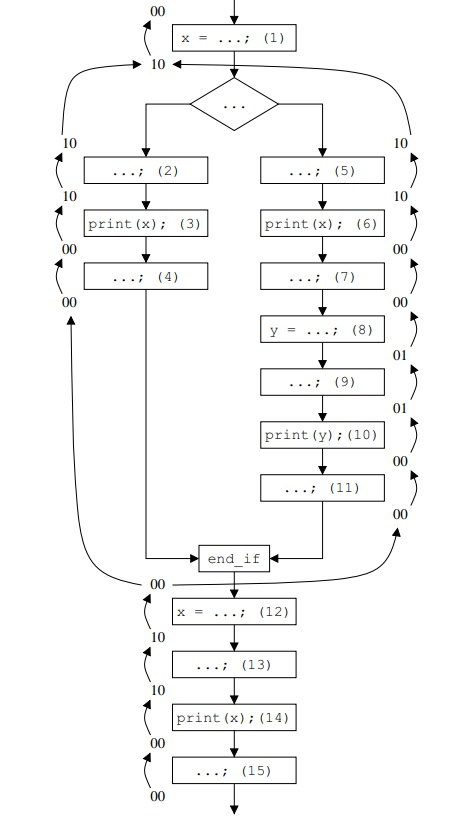
\includegraphics[scale=0.45]{525.jpg}
  \end{center}
\end{frame}

\begin{frame}
  \frametitle{Live analysis by data-flow equations}
  \begin{block}{Description}
\justify{The algoritm starts by setting the bits in the $OUT$ to 00: First because x does not live at the end of the scope and second because y even does not exist there.\\
Following the control-flow graph we find firs apperance of x and w set bits in out to 10. Following data equations algoritm finds out that $IN$ is 10.\\
The next step is assignment to x. This sets $GEN$ set to empty and $KILL$ set contains \textit{x lives there}. After applying the second data-flow equation the $IN$ set is set to 00.\\
Continuing this way, we propagate the bits upwards, splitting them at the end-if node and merging them at the if-node, until we reach the beginning of the block with the bits 00.} 
  \end{block}
\end{frame}

\begin{frame}
  \frametitle{Live analysis by data-flow equations}
  \begin{block}{Several observations}
\begin{itemize}
    \item The union in the data-flow equations can be implemented as a simple Boolean OR, since if a variable is live along one path from a node it is live at that node
    \item  It is important to note that the diagram does not contain the bit combination 11, so there is no node at which both variables are live. This means that they canshare the same register or memory location. Indeed, the live range of x in the right branch of the if-statement stops at the statement print(x+3) and does not overlap the live range of y.
    \item  The nodes with the last use of the value of a variable V can be recognized by having a 1 for the liveness of V in the $IN$ set and a 0 in the $OUT$ set.
\end{itemize}
  \end{block}
\end{frame}


\end{document}
